\chapter{Conclusion and Future Work}
\label{sec:conclusion_future_work}

\section{Conclusion}

This thesis examines the effectiveness of various expansion methods in approximating the probability density function of asset returns within the Heston stochastic volatility model. It begins by emphasizing the critical role of realized moments-including variance, skewness, and kurtosis—in derivative pricing and risk management. The literature review provides an overview of traditional approaches for estimating low-frequency moments from high-frequency data and introduces key expansion techniques, such as the Gram–Charlier and Edgeworth expansions, alongside alternative methods, including the Cornish–Fisher and Saddlepoint approximations.

At the core of this study is the Heston model, in which volatility is itself stochastic, evolving according to a mean-reverting process driven by correlated Brownian motions. The thesis addresses simulation challenges, particularly numerical instabilities that arise when the Feller condition is violated. A comprehensive simulation study is conducted over a large grid of parameter combinations using high-frequency data, with a rigorous filtering process to exclude simulations exhibiting numerical errors.

The empirical analysis evaluates the performance of different expansion methods, with a particular focus on the Gram-Charlier and Edgeworth expansions, by applying good\-ness-of-fit tests, including the Kolmogorov–Smirnov and Anderson–Darling tests. The findings indicate that cumulant-based methods generally produce more accurate approximations than moment-based approaches. However, while positivity constraints are essential to ensure valid probability densities, they introduce distortions in the estimated distributions. Furthermore, the study identifies that the quality of approximations is most sensitive to variations in the volatility parameter ($\sigma$) as well as the mean-reversion parameters ($\kappa$ and $\theta$).

Overall, the thesis concludes that incorporating higher-order cumulants substantially enhances the accuracy of return distribution approximations relative to the baseline normal model. These insights contribute to the refinement of pricing models and risk management strategies in financial applications.

\section{Future Work}

The numerical errors that occurred during the Heston model simulation using the Quadratic Exponential (QE) scheme were successfully identified and excluded. It was found that these errors arose when the Feller condition was strongly violated. However, Andersen (\citeyear{andersenEfficientSimulationHeston2007}) states in his paper that the QE scheme should remain valid even in such cases, suggesting that the issue was likely due to an implementation error. Indeed, by the end of this research, the source of the error was located and corrected. Unfortunately, time constraints did not allow for a full re-computation of the affected simulations. The problem was traced to the computation of Equation \eqref{eq:qe_dirac} and the sampling of $U_v$ from the uniform distribution. If $U_v$ exactly equaled 1, then the computation of $\Psi^{-1}$ resulted in a division by zero, leading to numerical failures. This issue only arose when $v_t$ was very small and remained so, which occurs when the Feller condition is significantly violated. The sampling range of $U_v$ was adjusted to lie between $10^{-10}$ and $1-10^{-10}$, which eliminated the error in preliminary tests. Future work should re-run the simulations with this adjustment to ensure that the QE scheme is correctly implemented.

\begin{figure}
    \centering
    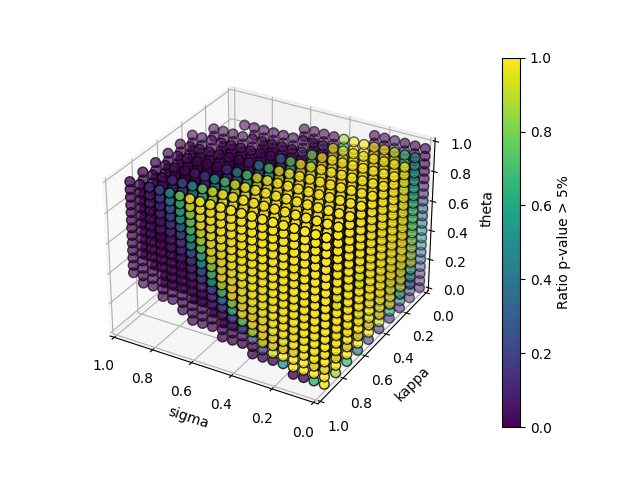
\includegraphics[width=0.8\textwidth]{img/GC_cum_KS_3d_p_value_sigma_kappa_theta.png}
    \caption{Percentage of simulations where the p-value of the Kolmogorov-Smirnov-Test against the theoretical density is above 5\%. Invalid simulations are excluded. $\mu=0.05$.}
    \label{fig:GC_cum_KS_3d_p_value_sigma_kappa_theta_mu005}
\end{figure}

A more detailed comparison between the cases $\mu = 0$ and $\mu = 0.05$ can be observed in Figure \ref{fig:GC_cum_KS_3d_p_value_sigma_kappa_theta_mu005}, which highlights the differences more clearly than the previous 3D visualization for $\mu = 0$ (Figure \ref{fig:GC_cum_KS_3d_p_value_sigma_kappa_theta_muzero}). It remains unclear why the Gram-Charlier expansion produces better approximations in certain cases when $\mu = 0.05$, and whether this effect persists for other values of $\mu$. This presents a potential avenue for future research.

A similar trend would be observed in a pair plot analogous to Figure \ref{fig:pairplot_GC_cum_KS_muzero}, further reinforcing the pattern: there are more yellow regions in the pair plot for $\mu = 0.05$, suggesting that, for suitably chosen parameters, the Gram-Charlier expansion better approximates the theoretical distribution when the price process is not a martingale. However, this improvement is counterbalanced by a higher number of parameter combinations—particularly in $\sigma$, $\kappa$, and $\theta$—where the Gram-Charlier expansion performs worse in approximating the theoretical distribution.

More generally, expanding the parameter ranges could provide deeper insights. This study considered only a limited subset of the possible parameter space. A broader exploration may reveal scenarios where positivity-constrained expansion methods outperform their unconstrained counterparts, particularly in cases where the unconstrained cumulant expansions produce negative densities.